\documentclass[12pt]{article}
\usepackage{graphicx}
\usepackage {color}
\usepackage{pdfpages}
\usepackage{float}
\usepackage{changebar}
\usepackage{enumitem,amssymb}
\renewcommand{\familydefault}{\sfdefault}
\usepackage[margin=1.2in]{geometry}
\usepackage{graphicx}
\usepackage{wrapfig}
\usepackage[super]{cite}
\usepackage{subcaption}
\usepackage[table]{xcolor}
\usepackage{amsmath}
\usepackage[sort, numbers]{natbib}

%%%%%%%%%%%%Defining the margins %%%%%%%%%%%%%%%%%%%%%
\textheight 9.in
\textwidth 6.5in
\topmargin -.5in
\oddsidemargin 0in
\setlength{\parskip}{\smallskipamount}

%%%%%%%%%%%%%%Specific Commands %%%%%%%%%%%%%%%%%%
\newcommand{\eg}{{\em e.g.,}}
\newcommand{\ie}{{\em i.e.,}}
\newcommand{\etc}{{\em etc.,}}
\newcommand{\etal}{{\em et al.}}
\newcommand{\degrees}{{$^{\circ}$}}
\newcommand{\fig}[1]{\textbf{Figure #1}}

%%%%%%%%%%%%%%%%%%%%%%%%%%%% Setting to control figure placement
% These determine the rules used to place floating objects like figures 
% They are only guides, but read the manual to see the effect of each.
\renewcommand{\topfraction}{.9}
\renewcommand{\bottomfraction}{.9}
\renewcommand{\textfraction}{.1}
\renewcommand{\familydefault}{\sfdefault} %setting the san serif font

%%%%%%%%%%%%%%%%%%%%%%%% Line spacing
% Use the following command for ``double'' spacing
%\setlength{\baselineskip}{1.2\baselineskip}
% and this one for an acceptable NIH spacing of 6lpi based on 11pt
%\setlength{\baselineskip}{.9\baselineskip}
% The baselineskip does not appear to work when we include a maketitle
% command in the main file.  Something there must set the line spacing
% If we use this next command, then things seem to work.
\renewcommand{\baselinestretch}{.9}

\setcounter{secnumdepth}{0} %make no numbers but have a table of contents


\begin{document}

\title{Lab 4, Neuron and Backyard Brains}
\author{Jake Bergquist, u6010393}
\maketitle
\tableofcontents
\newpage

\section{Introduction}
\par{}
For this labratory assignment we experimented with a Neuron model of a cardiac atrial myocyte developed by Courtemanche \etal{} \cite{Courtemanche1998} Cardiac Myocytes are the cells responsible both for propagating the electrical signals through the heart as well as performing the mechanical action of pumping the blood. Atrial myocytes in particular are responsible for pumping blood from the left and right atria into the left and right ventricles respectively. While the mechanical capabilities of the atrial myocytes are relativly little compared to the ventricles, the electrical role these atrial myocytes perform is critical to the function of the heart. The electrical signal that initiates a heartbeat begins in the atria at the sino-atrial node. The atrial myocytes then propagate this electrical signal across the atria to the atrio-ventricular node where the electrical signal then goes on to activate the rest of the heart and initiate the rest of the heart beat. The signals from the atrial myocyte activations comprise the 'P' wave of the QRS complex of an electro cardiogram. Without functioning atrial myocytes the electrical signal to the atria and thus the rest of the heart would be disturbed, potentially leading to dangerous and sometimes fatal conditions such as atrial fibrillation, arrhythmias, and other cardiac diseases.
\par{}
The atrial myocyte model we used allowed for manipulation of many different parameters. The simulation is set up the stimulate at a regular interval to initiate an action potential periodically, then plot membrane voltage over the simulation. The parameters chosen for this study were the three conductances most important to the cardiac action potential, the sodium, potassium, and calcium conductances. For each conductance we tested the model at the baseline level, then at double conductance, then at half conductance. These conductances are affected in many disease states, leading to various heart diseases and malfunctions, and our manipulations resemble variations seen in disease states where conductances are increased or decreased.\cite{DaFaria2008} We utilized the backyard brains spike recorder and a custom matlab script to inject current into and record from an agar block. In addition to varying the simulation parameters of the three conductances we also varied the recording locations on the agar block. Additionally we tested the effects of multiple simulations at nearby locations in the agar.
\par{}
The intracellular effects of these simulation manipulations were apparent in the membrane voltage plots, and the ionic current plots. Changes to the sodium conductance affected the upstroke of the membrane potential during the action potential as well as the initial phase of the sodium current. As expected, increased conductance resulted in a higher peak voltage while lower conductance resulted in a reduced peak. The peak duration however was not affected as sodium channels are time inactivated and thus the conductance does not affect the peak duration. These changes were reflected in the current plots with a higher sodium current peak. When potassium was adjusted this primarily affected the repolarization stage, where the potassium current brings the membrane voltage back towards the resting potential. Increasing potassium conductance caused an increase in potassium current which resulted in a shorter plateau phase and a more rapid repolarization. Decreasing the potassium had the opposite effect, increasing plateau time and slowing repolarization. Changing calcium should also affect the repolarization and plateau phases of the  cardiac action potential. Calcium is responsible for sustaining the plateau phase, thus reducing calcium, thereby reducing the calcium current, resulted in a decreased plateau time and more rapid repolarization. Increasing calcium conductance increased the plateau time and delayed the repolarization. These results fit our understanding of an atrial myocyte.
\par{}
We would predict to see these changes reflected in the extracellular recordings however the actual effects were difficult to interpret. Changes in recording location did affect the resulting signals recorded. When the recording was taken from electrodes that were adjacent to the stimulation the amplitudes were less than when the recording was from electrodes across the stimulated area. Additionally, stimulating with two different parameter sets next to each other gave a unique signal that seems different from either one individually. However the specific changes predicted by the ion conductance variations described above were not necessarily reflected. This could be the result of several factors which are explored in the results and discussion section of this report


\section{Methods}
\subsection{Hardware Setup}
\par{}
The backyard brain recording device was plugged into a laptop running the spike recorder software, and the recorder was linked to the software. The headphone wires were plugged into the audio jack of the laptop which also had the custom matlab script loaded. This setup can be seen in \ref{fig:setup} where the blue agar block was our conductive medium. All recordings referencing position one were made using ground (top electrode) and position one (middle electrode). All recordings referencing position two were made using the ground (top electrode) and position two (bottom electrode). The headphone wires were placed a few millimeters into the agar block as seen in \ref{fig:setup}. By using matlab a sound file generated by the neuron model could be used to pass current into the agar according to the neuron simulation. The headphone wire positions were held constant. The bandpass filter cutoff frequencies were set to 1 hz and 50 hz, and the attenuation was set to 60 hz (these are the default parameters when the backyard brains hardware is synced to the spike recording software).


\begin{figure}[H]
	\centering
	\centering
	\includegraphics[width = .95\textwidth]{setup.png}
	
	\caption{Our hardware setup. The top electrode was connected to the ground lead of the backyard brains spike recorded while the other two electrodes were used as our variable positions. The topmost electrode is referenced as ground, the middle electrode is position 1, and the bottom electrode is position 2. The headphone wires embedded into the agar block delivered the simulation currents. These currents were generated by playing the simulation as a converted audio file via custom matlab function. }
	\label{fig:setup}
\end{figure}
\par{}

\subsection{Simulation Parameter Setup}
\par{}
During this lab we varied the conductances of the three most important ions that shape the action potential of cardiac myocytes: sodium, potassium, and calcium. For each of these ions we tested an increased conductance (doubled), a decreased conductance (halved), and a baseline conductance. These values can be seen in \ref{tab:conductances}. All other parameters including the stimulation parameters were left at default values as described in Courtemanche \etal{}\cite{Courtemanche1998} For each case only one parameter was changed at a time.

 \rowcolors{2}{gray!25}{white}
\begin{table}[H]
	\centering
	\caption{Simulation parameters used for exploration. The three main ion conductances, Sodium, Potassium, and Calcium, were adjusted to see their effects on the action potential and currents.}
	\label{tab:conductances}
	\begin{tabular}{cccc}
		\hline \hline
		Ion  & Default Conductance & Double Conductance & Half Conductance\\ 
		\hline
		Calcium (gCaL)& 0.248 $S/cm^2$&0.496 $S/cm^2$& 0.124 $S/cm^2$\\ 
		Potassium (Ikr) & 5.88 $S/cm^2$ & 11.76 $S/cm^2$& 2.94 $S/cm^2$\\ 
		Sodium (NaBar)& 0.156 $S/cm^2$ & 0.312 $S/cm^2$ & 0.078 $S/cm^2$\\ 
		\hline 
		\hline
	\end{tabular} 
\end{table}
\subsection{Stimulation Generation and Recording}
\par{}
For each simulation output the timescale was zoomed in onto the last action potential of the simulation, between 40,000 ms and 41,000 ms into the simulation.
\par{}
For each conductance change first the simulation was run in Neuron and the membrane voltage and ionic currents (for sodium, potassium, and calcium) were plotted. The current vectors were then saved out individually, and a custom matlab script was used to integrate these current signals and pass this over the headphone jack. Form most recordings the same signal was passed through the headphones. For each conductance value perturbation we measured from ground to position 1. Additionally we tested the effect of interfering signals by recording from ground to position 2 and playing a double calcium conductance signal though one wire and a half calcium conductance signal through the other. This allowed us to assess the ability to detect these different signals using the surface recording electrodes given the interference between the signals. For all of these recordings we compared our recorded signals both to the expected transmembrane potentials from our simulation as well as to the baseline recordings. Finally we recorded the baseline simulation at both recording locations to assess the effect of recording location on the signals obtained. 

\section{Results and Discussion}
\subsection{1: Manipulation of parameters and their effect on cellular electrical  propagation}
\par{}
First we must consider the simulation results of our baseline parameter set. This can be seen in \ref{fig:baseline} which shows the expected basic cardiac action potential, with a sharp upstroke, prolonged plateau and then repolarization. We will use this simulation result as a basis for comparison when we manipulate the parameters of the simulations.
\par{}
By design we manipulated the conductances that we expected would have a marked effect on the cardiac action potential. First considering the Sodium conductance. Sodium is responsible for the upstroke during initial depolarization of the action potential. When we double this conductance we expect to see an increase in the action potential peak during the upstroke, but no change in the upstroke/sodium current duration. This can be seen in \ref{fig:doubleNa} where the action potential peak is increased to about 45 mV as compared to the 25 mV peak seen in the baseline plot. Additionally the sodium current is nearly doubled in comparison to the baseline. This agrees with our understanding of the function of the sodium conductance in the myocardial cell. 


\begin{figure}[H]
	\centering
	\centering
	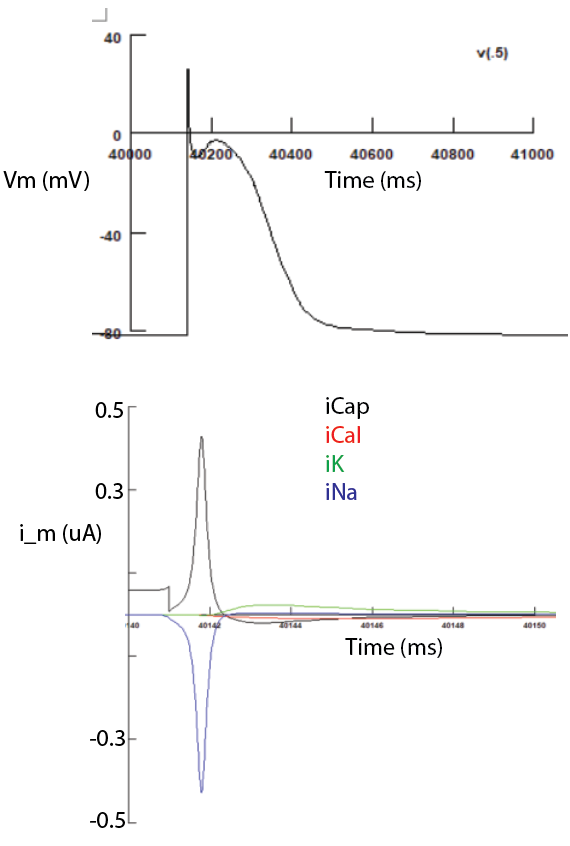
\includegraphics[width = .95\textwidth]{OriginalSimulation.png}
	
	\caption{This figure shows the simulation results given the default parameters. As can be seen the membrane voltage shows a typical myocardial action potential. The second plot shows the expected currents for such an action potential. }
	\label{fig:baseline}
\end{figure}
\begin{figure}[H]
	\centering
	\centering
	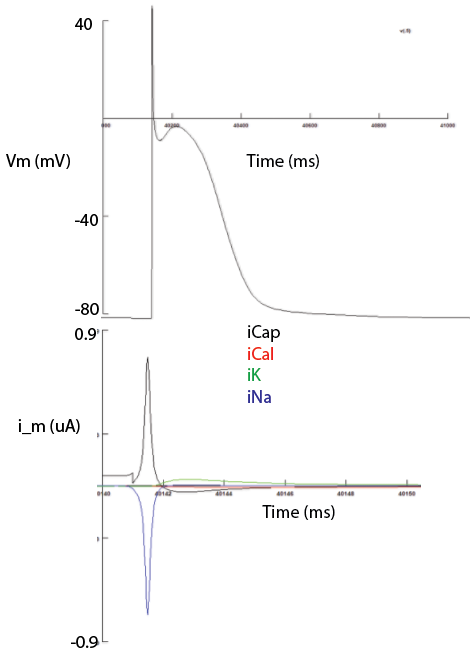
\includegraphics[width = .95\textwidth]{DoubleNaSimulation.png}
	
	\caption{This figure shows the simulation results with the baseline sodium conductance doubled according to Table 1. As can be seen the membrane voltage shows a myocardial action potential with an increased peak voltage. The second plot shows the expected currents for such an action potential with an increased sodium peak. Note the different scale as compared to the baseline. }
	\label{fig:doubleNa}
\end{figure}
\begin{figure}[H]
	\centering
	\centering
	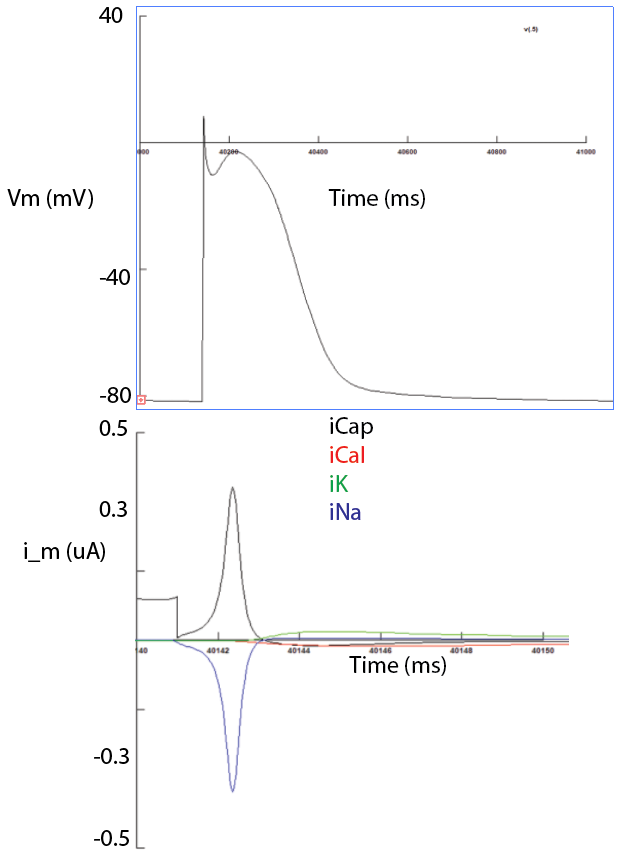
\includegraphics[width = .95\textwidth]{HalfNaSimulation.png}
	
	\caption{This figure shows the simulation results with the baseline sodium conductance halved according to Table 1. As can be seen the membrane voltage shows a myocardial action potential with an decreased peak voltage. The second plot shows the expected currents for such an action potential with an decreased sodium peak. }
	\label{fig:halfNa}
\end{figure}

\par{}
Next we consider the potassium conductance. Potassium plays a role in repolarization. Potassium drives the repolarization after sodium channel activation and the combination of potassium and calcium currents dictate the plateau phase of the cardiac action potential. Increasing this conductance should result in an increased repolarization response, which should in turn cause a more rapid downslope and shorten the plateau phase. We see these expected results in \ref{fig:doubleK} as the increased potassium conductance results in an increased potassium current during the repolarization, and a decreased plateau phase. As expected these results are reversed in the half potassium conductance trials. A decreased potassium conductance is seen in diseases where repolarization is not as robust. As expected, in this trial the decreased potassium conductance resulted in a prolonged plateau and delayed repolarization to resting potential. However because there is still some potassium conductance the cell does indeed still repolarize eventually. The time to repolarization however is almost double compared to the increased potassium conductance. These results are shown in \ref{fig:halfK}.

\begin{figure}[H]
	\centering
	\centering
	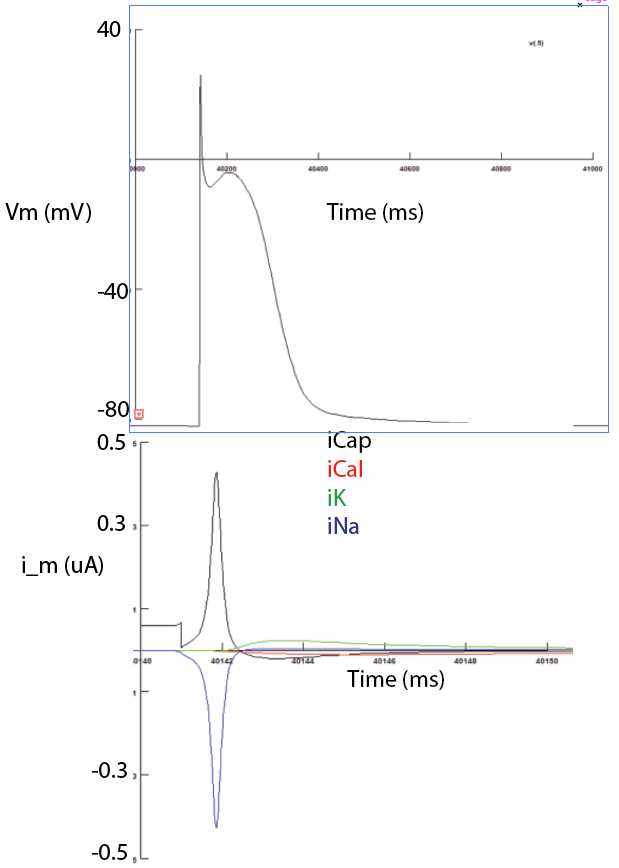
\includegraphics[width = .95\textwidth]{DoubleKSimulation.png}
	
	\caption{This figure shows the simulation results with the baseline potassium conductance doubled according to Table 1. As can be seen the membrane voltage shows a myocardial action potential with an increased and earlier repolarization slope and decreased plateau duration. The second plot shows the expected currents for such an action potential with an increased potassium current. }
	\label{fig:doubleK}
\end{figure}
\begin{figure}[H]
	\centering
	\centering
	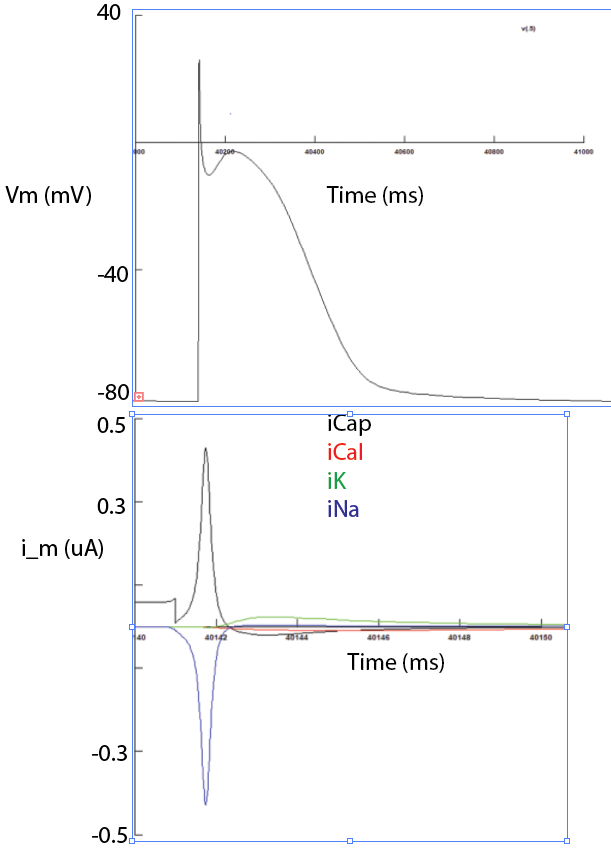
\includegraphics[width = .95\textwidth]{HalfKSimulation.png}
	
	\caption{This figure shows the simulation results with the baseline potassium conductance halved according to Table 1. As can be seen the membrane voltage shows a myocardial action potential with an decreased and delayed repolarization slope and increased plateau duration. The second plot shows the expected currents for such an action potential with an increased potassium current. }
	\label{fig:halfK}
\end{figure}


\par{}
Finally we manipulated the calcium conductance, which is the primary driving ion during the plateau phase of the action potential. Calcium currents maintain the membrane voltage during the plateau despite the potassium repolarizing current. Increases in calcium conductance cause a striking change in the repolarization phase in our simulation of the trans membrane voltage seen in \ref{fig:doubleCa}. Here we can see that the plateau voltage is raised above zero and the plateau is sustained but not for as long as we might expect. This is because calcium channels are only active for a certain amount of time, and the cell still rapidly repolarizes due to potassium and other currents after this time. Again when we perform the reverse manipulation, halving the calcium conductance, we see a reverse result in the simulation. In this case \ref{fig:halfCa} shows a decrease in the plateau amplitude and the plateau duration. The decrease in duration results from the potassium current being able to more quickly overtake the calcium current due to the reduced calcium conductance.

\begin{figure}[H]
	\centering
	\centering
	\includegraphics[width = .95\textwidth]{DoubleCaSimulation.png}
	
	\caption{This figure shows the simulation results with the baseline calcium conductance doubled according to Table 1. As can be seen the membrane voltage shows a myocardial action potential with an increased time to repolarization and increased plateau duration as well as amplitude. The second plot shows the expected currents for such an action potential with a increased calcium current. }
	\label{fig:doubleCa}
\end{figure}
\begin{figure}[H]
	\centering
	\centering
	\includegraphics[width = .95\textwidth]{HalfCaSimulation.png}
	
	\caption{This figure shows the simulation results with the baseline calcium conductance halved according to Table 1. As can be seen the membrane voltage shows a myocardial action potential with an decreased time to repolarization and decreased plateau duration. The second plot shows the expected currents for such an action potential with a decreased calcium current. }
	\label{fig:halfCa}
\end{figure}

\subsection{2: How do the simulation results change as we manipulate the parameters within physiological ranges and what explains these changes? }
\par{}
In the field of cardiac electrophysiology conductance parameters are usually expressed according to S/F \cite{TenTusscher2003} however this model used units of S/cm2. However it is reasonable to expect to see conductances that are roughly half their baseline values in certain disease states.\cite{DaFaria2008} Doubled conductances however are typically out of range for normal physiological conditions even in disease states. The resulting changes of the simulation are described above. When we look at these results in our recorded data (\ref{fig:recNa}, \ref{fig:recK},\ref{fig:recCa}) it is difficult to see the expected variations. In the case of the sodium recordings, between the noise and baseline drift of the recordings it is difficult to discern if the trends we see are indeed real or just artifact, however in some cases it would seem that the increased sodium seems to have a higher upstroke peak than control and the decreased sodium with a lower. These results however are far less striking than the intracellular simulation recordings.
\par{}
The same trend is seen in the Potassium recordings where noise and drift complicate our analysis. In general we can say that there seems to be a reduced repolarization in the half potassium conductance recordings as expected. The increased potassium conductance recordings also seem to show some trend of hyperpolarization but this is difficult to actually describe given the poor quality of the signals.
\par{}
In the case of the calcium conductance recordings we see that an increase in calcium conductance does seem to raise the extracellular voltage after the initial spike as compared to baseline while the reduced calcium conductance has the opposite effect. Overall these recorded results illustrate the difficulty of translating electrical recordings directly to single cellular measures and vise versa. The reasoning for observed changes that could be identified in the recordings as well as all of the changes seen in the  simulations are well described in the previous section.
\subsection{3: Explain the relationship between intracellular potential and extracellular measured potential and explain what can be done to ensure the best recorded signal}
\par{}
In the field of cardiac electrophysiology typically measurements are taken on an organ level of extracellular voltage. This voltage of course originates in the individual cells as there are no electrically active components of the extracellular space that we know of in the heart. So often these recordings are seen as a sort of proxy for examining the cellular potentials, but this is not the whole picture. Considering a single cardiac myocyte, during the upstroke of its action potential a waveform is generated , as can be seen in our recordings. The polarity of this waveform depends on the orientation of the recording electrodes in relationship to the cell. After the upstroke there is a short down stroke caused by initial potassium conductance before calcium conductance kicks in to cause the plateau. This initial repolarization before the plateau causes another wave of the opposite sign of the initial wave on our recording electrodes. When the cell reaches the plateau phase, we see an isoelectric period in our recordings as no electrical changes are occurring to be recorded. Finally when repolarization occurs we see another waveform of the opposite sign of the initial waveform, indicating a cellular change in voltage opposite of the initial upstroke of the action potential. In this way the recording of electrical potentials extracellularly can inform us about intracellular voltage, but we must be careful to consider the location, orientation, and polarity of our recordings.
\par{}
To attempt to improve our signal recording we made sure to record near to the insertion of the wires, and played signal from both wires to amplify the signal we were trying to record. The hardware of the spike recorder likely applies some forms of amplification and possibly active filtering. On the software side we utilized the built in 60 hz attenuation filter to remove as much of the ambient 60 hz power noise as possible, as well as the built in 1 hz to 50 hz notch filter to exclude any frequencies not relevant to our recordings. We also could have utilizer a software such as PFEIFER to perform baseline correction and filtering to remove any non standard signals, but we opted not to in order as we deemed that the benefit gained from this would be minimal given our signals. Another approach would be to signal average across multiple stimulations in the same simulation, however doing so would require time alignment of the signals which is a computationally difficult or manually intractable problem when considering more than just a handful of signals.
\par{}
We also manipulated the recording electrode placement, as seen in \ref{fig:recPos} and found that at some electrode orientations we achieved vastly different signals. One possible explanation for this phenomena is that position one is adjacent to the stimulation site but the path between the electrode and ground is not over the stimulation site, whereas position 2 creates a path that directly crosses the wire insertion point, resulting in dramatically increased signals. However this did not account for the strange morphology of the signals recorded from position 2, and thus we feel that there must be something going on with this recording site that we are unsure how to explain. There is clearly still an initial two waves seen by the electrode corresponding to the initial sodium driven upstroke and the foloowing short potassium downstroke before the plateau, but we do not see any real plateau phase nor do we see a repolarization wave. This may be due to the orientation of this recording site or some other factors unaccounted for by our analysis.
 Despite this, the difference between the two recording sites highlights the need to consider recording position and orientation when designing experimental recordings of cardiac tissue.

\subsection{4: Describe what happens when different signals are played from each wire and what implications this has}
\par{}
For this trial, the results of which can be seen in \ref{fig:recInterfere}, we used the two calcium conductance change signals, one on each wire and recorded from position 2. From the recorded signals we can clearly see that the interference signal is different from baseline, but based on that signal alone, diagnosis would be impossible. This raises an important problem that detecting cellular level differences is very difficult from non direct extracellular recordings, especially when multiple cells can be exhibiting conflicting signals. Especially with only one electrode it is daunting to try and image a way to reconstruct the individual signals of each of these two "cells". Thus when designing experiments we must account for these limitations in our experimental designs and create experimental designs based on the specific goals we have. If we were to want to reconstruct these individual cells, at least two recordings, but preferably more from several sites around the cells, would be desired to parse out the individual cell contributions. These considerations are what drive the experimental design of cardiac electrophysiological research.

\subsection{5: Describe what magnitude of change of the simulation parameters is required to produce identifiable changes in the extracellular recording. What kinds of limitations might this suggest for experiments or clinical application?}
\par{}
In order to see even minor changes in the recorded signals we needed to make very aggressive changes to the model parameters given our recording location. Changing each conductance to double or half often produced a visible result on the recorded signals, but in most cases this change was far less than expected. Perhaps more detailed analysis of the recording location could have revealed an orientation of recording that optimized the detection of these differences however in the orientation we used only large changes produced a visible effect. Thus any smaller changes would have gone un noticed. In the context of experimental or clinical applications, this stresses the importance of proper recording location selection and understanding. This also suggests that small changes in cellular activity that are clearly visible on a cellular level, could easily go un noticed or marked off as noise or artifact in both experimental and clinical settings. This severely limits the application of signals collected this way in how they can be used to understand and diagnose cellular level phenomena. To alleviate this care must be taken to optimize the recording of these signals. This would likely mean using a larger number of more sensitive electrodes in a well designed orientation to answer the desired questions. These design features must be carefully considered by clinicians and researchers working with such signals.
\section{Conclusions}
\par{}
The cell model utilized is very similar to ones used previously in class such as the Ten Tusscher myocyte model. \cite{TenTusscher2003} The calculated currents and potentials agree well between the models however the currently examined model is fit specifically to an atrial cell and has many more specific and relative characteristics of that cell type. Overall we conclude from this study that the model used does indeed display the expected results from manipulation of the ion conductances that drive the cardiac myocyte action potential. We were able to explore changes in these ionic conductances as well as any other parameter in the model and the effect on the atrial myocyte action potential. Additionally we find that many changes made on a single or even two cell level may be exceedingly difficult to detect utilizing extracellular recordings. Additionally extracellular recordings add the additional considerations of dealing with noise, artifact, electrode arrangement and number, as well as the particular properties of the surrounding tissue. All of these must be taken into account when studying cellular recordings on a tissue level and even for studying tissue recordings.





\section{Figure Appendix}
\begin{figure}[H]
	\centering
	\centering
	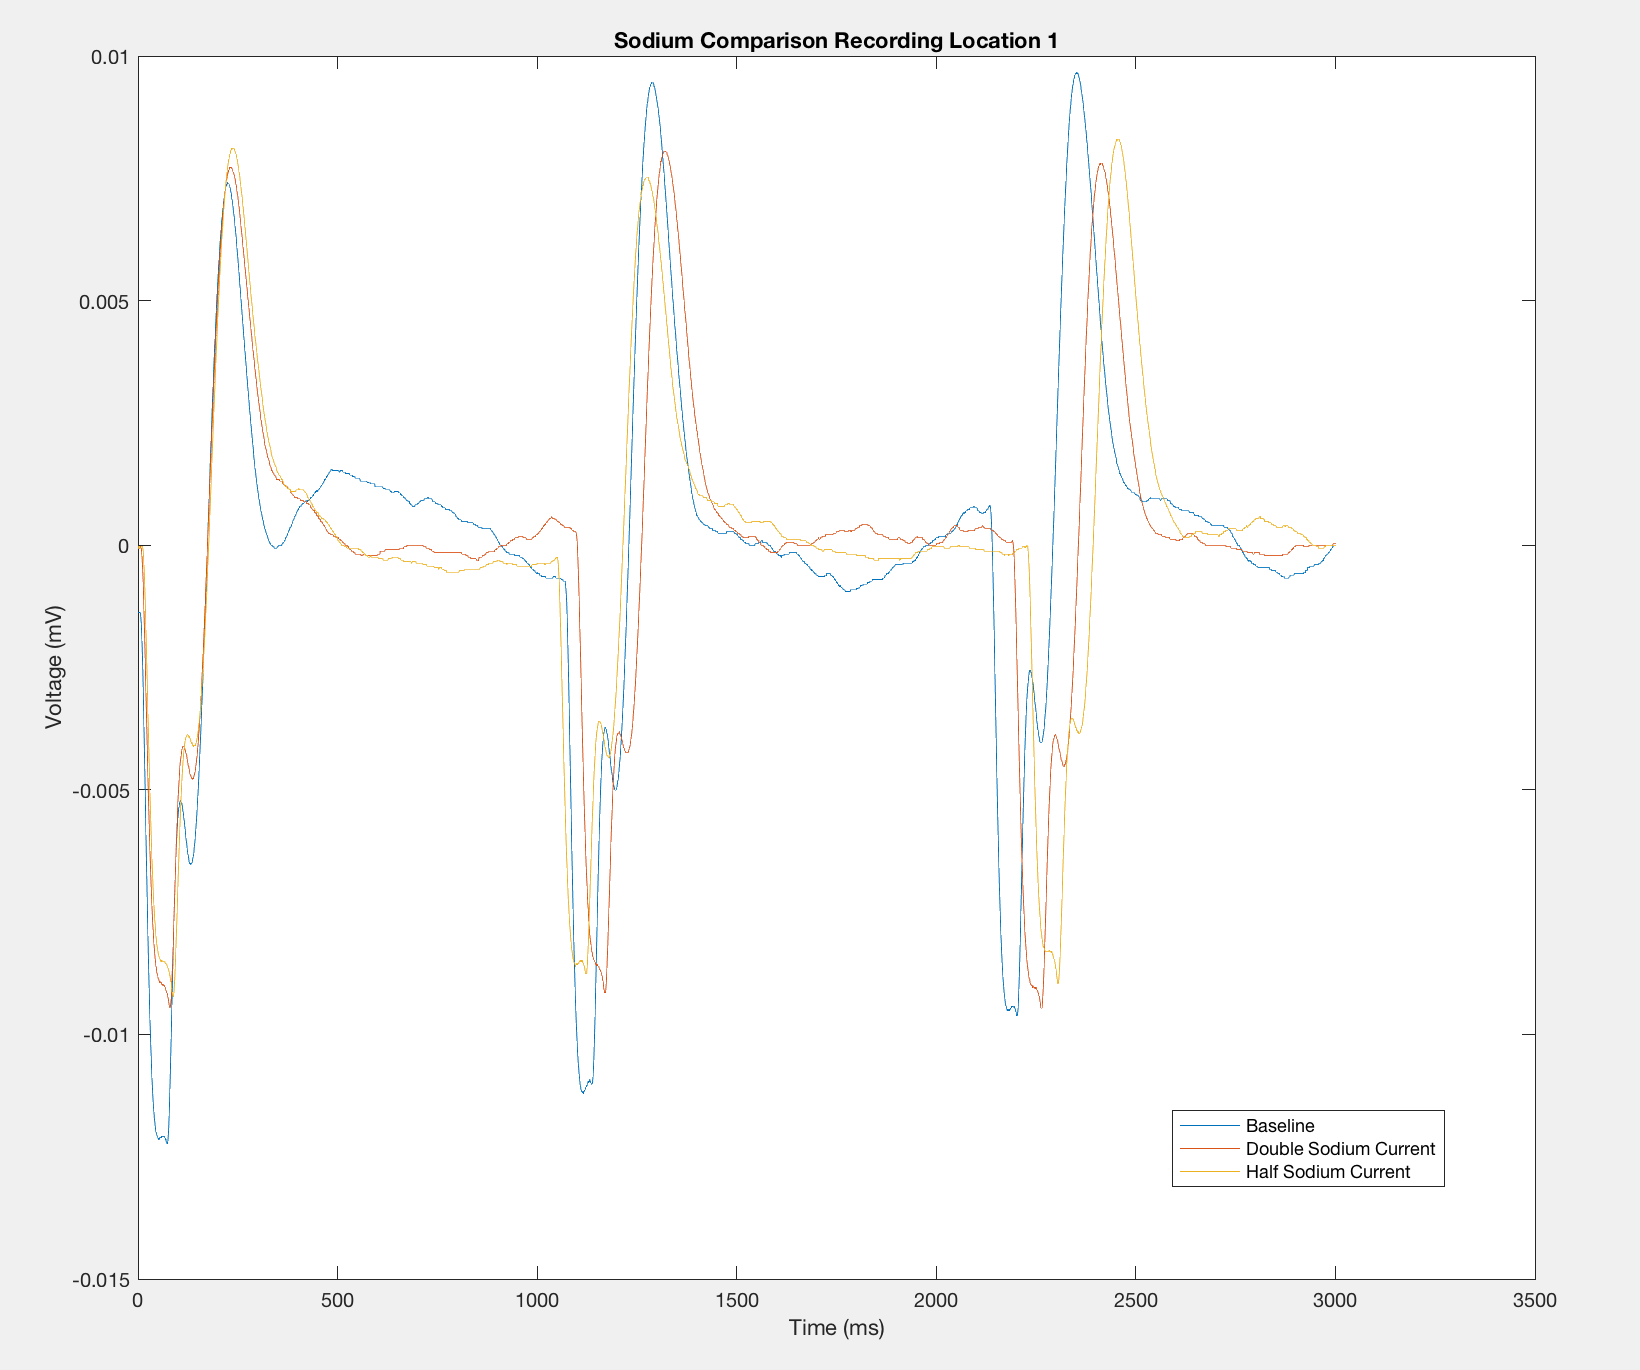
\includegraphics[width = .95\textwidth]{RecSodium.png}
	
	\caption{This figure shows the recording results with the different sodium conductance values according to Table 1. Baseline in Blue, double conductance in Red, half conductance in Yellow. X axis is time in ms and y is voltage in mV  }
	\label{fig:recNa}
\end{figure}
\begin{figure}[H]
	\centering
	\centering
	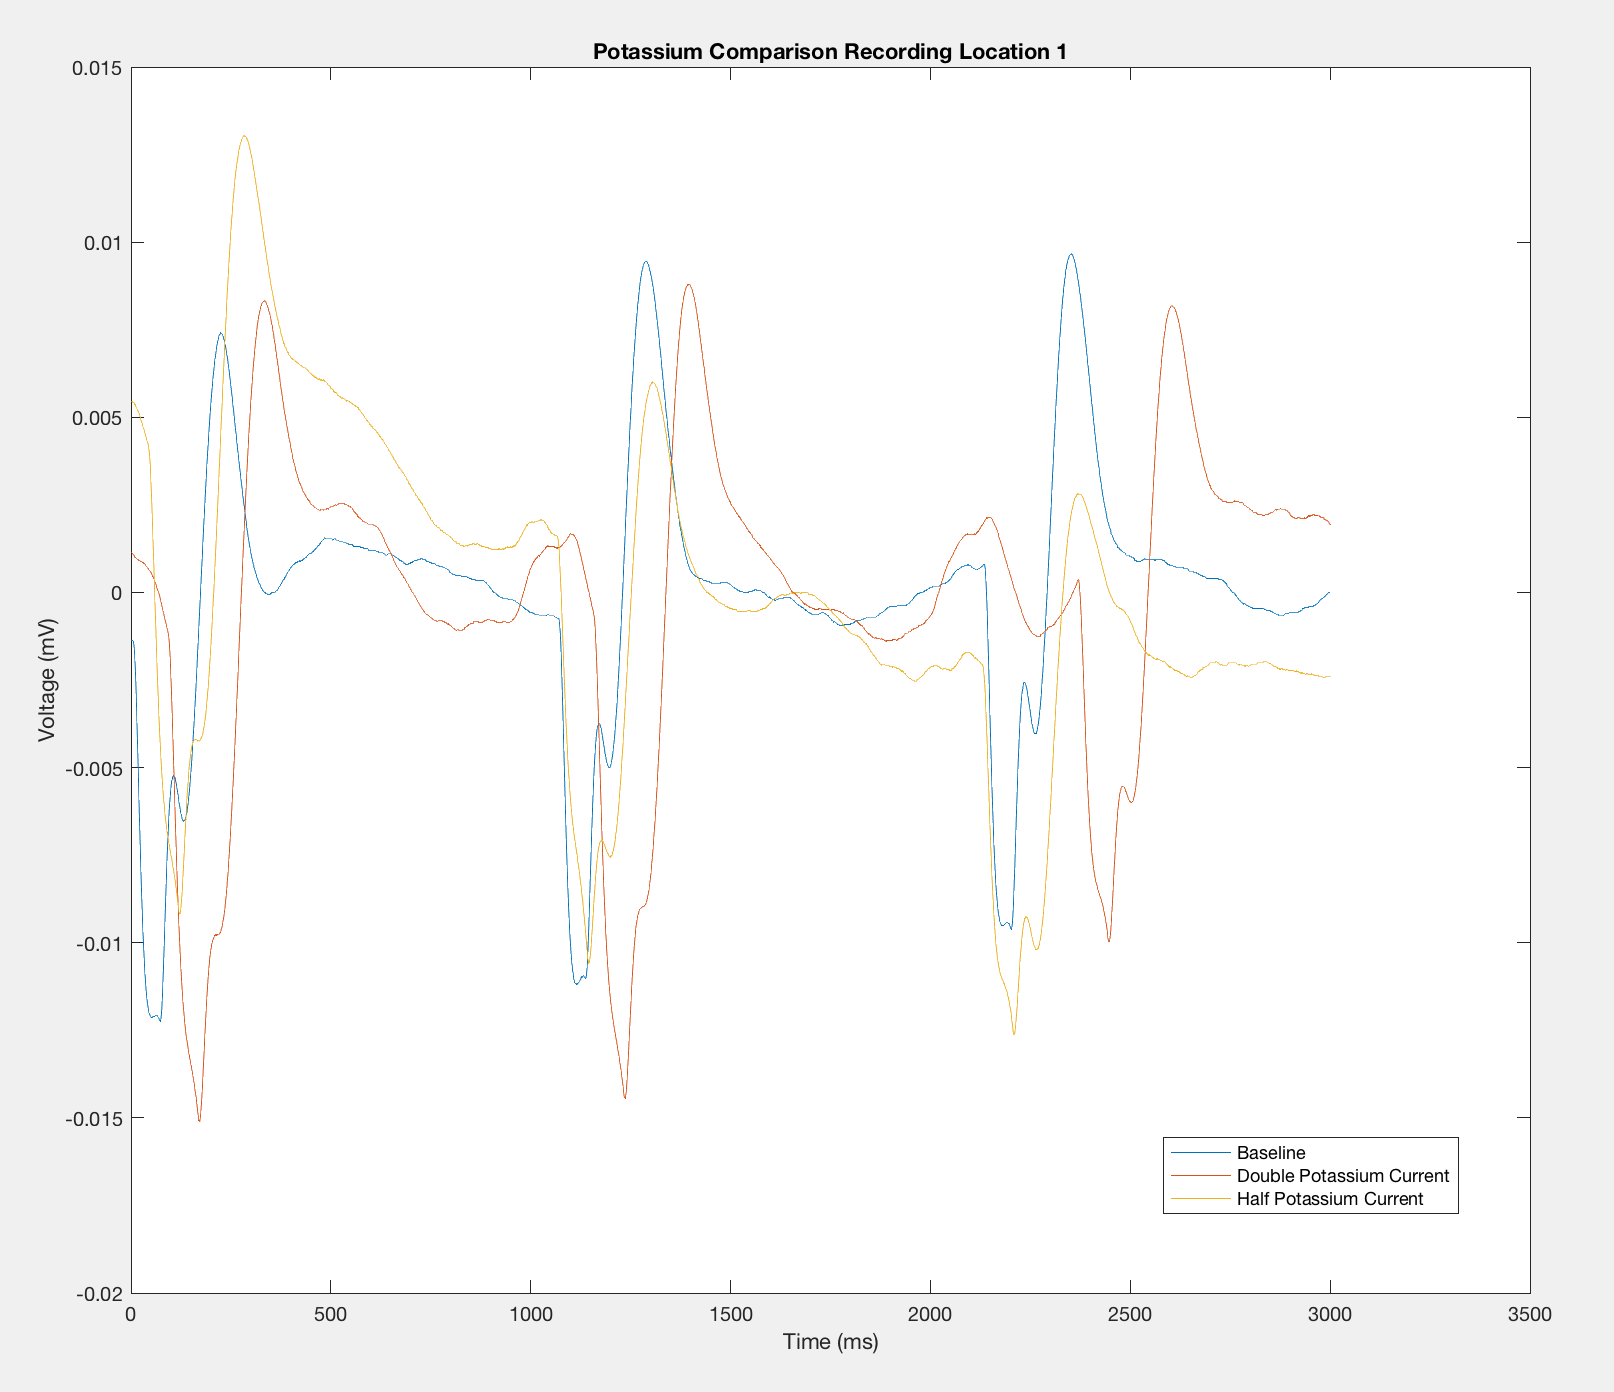
\includegraphics[width = .95\textwidth]{RecPotassium.png}
	
	\caption{This figure shows the recording results with the different potassium conductance values according to Table 1. Baseline in Blue, double conductance in Red, half conductance in Yellow. X axis is time in ms and y is voltage in mV  }
	\label{fig:recK}
\end{figure}
\begin{figure}[H]
	\centering
	\centering
	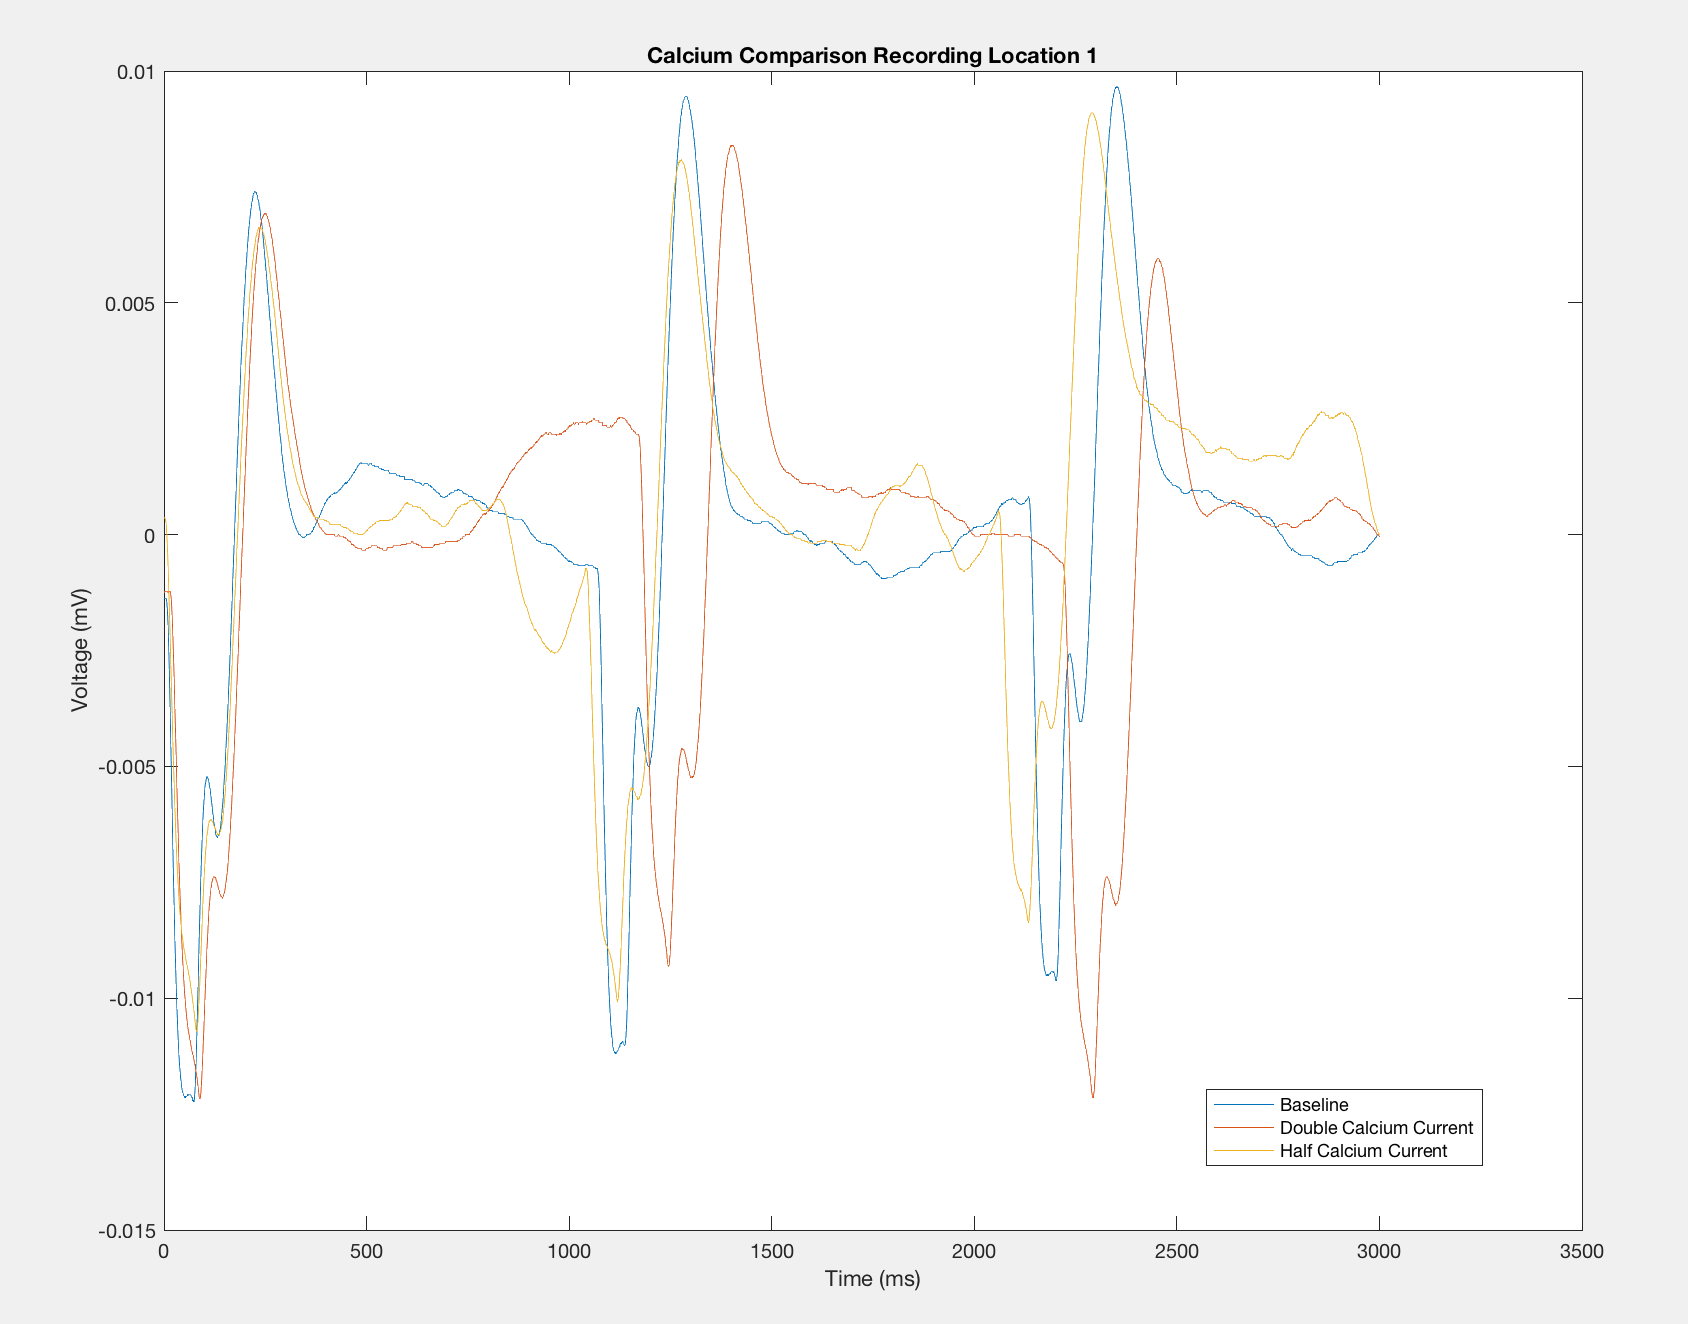
\includegraphics[width = .95\textwidth]{RecCalcium.png}
	
	\caption{This figure shows the recording results with the different calcium conductance values according to Table 1. Baseline in Blue, double conductance in Red, half conductance in Yellow. X axis is time in ms and y is voltage in mV }
	\label{fig:recCa}
\end{figure}
\begin{figure}[H]
	\centering
	\centering
	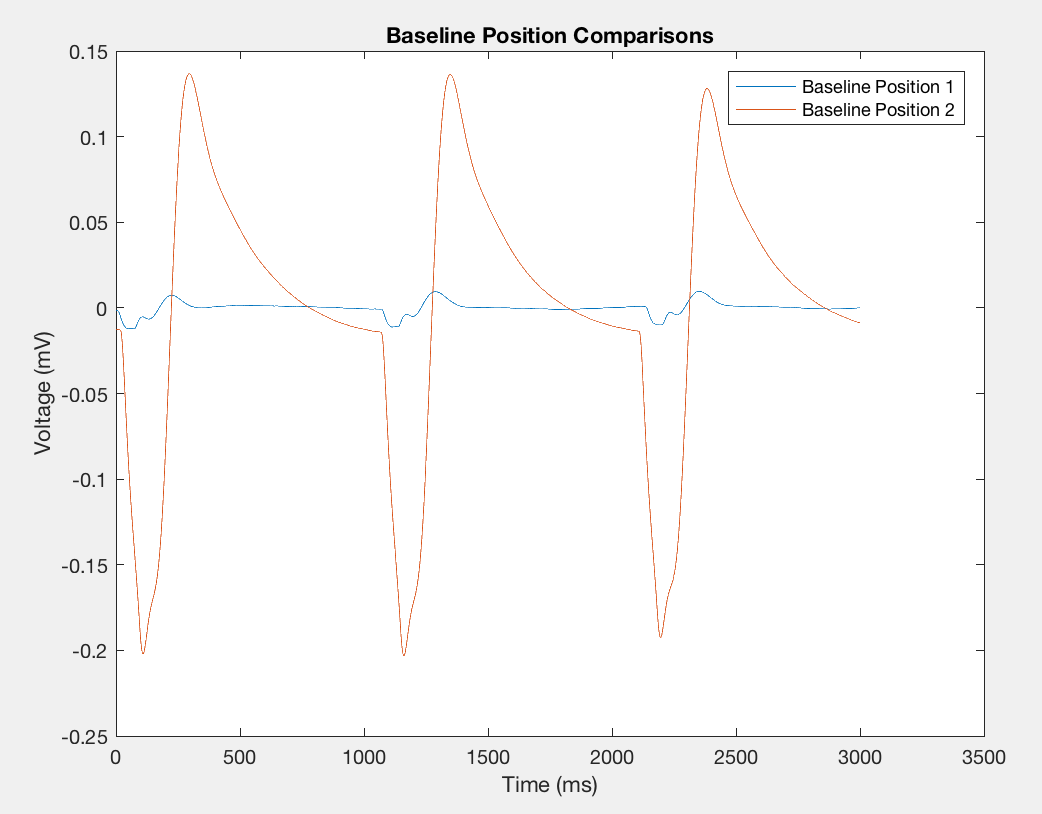
\includegraphics[width = .95\textwidth]{RecPositions.png}
	
	\caption{This figure shows the recording results with the different recording locations.  Position 1 in Blue, position 2 in Red. X axis is time in ms and y is voltage in mV}
	\label{fig:recPos}
\end{figure}
\begin{figure}[H]
	\centering
	\centering
	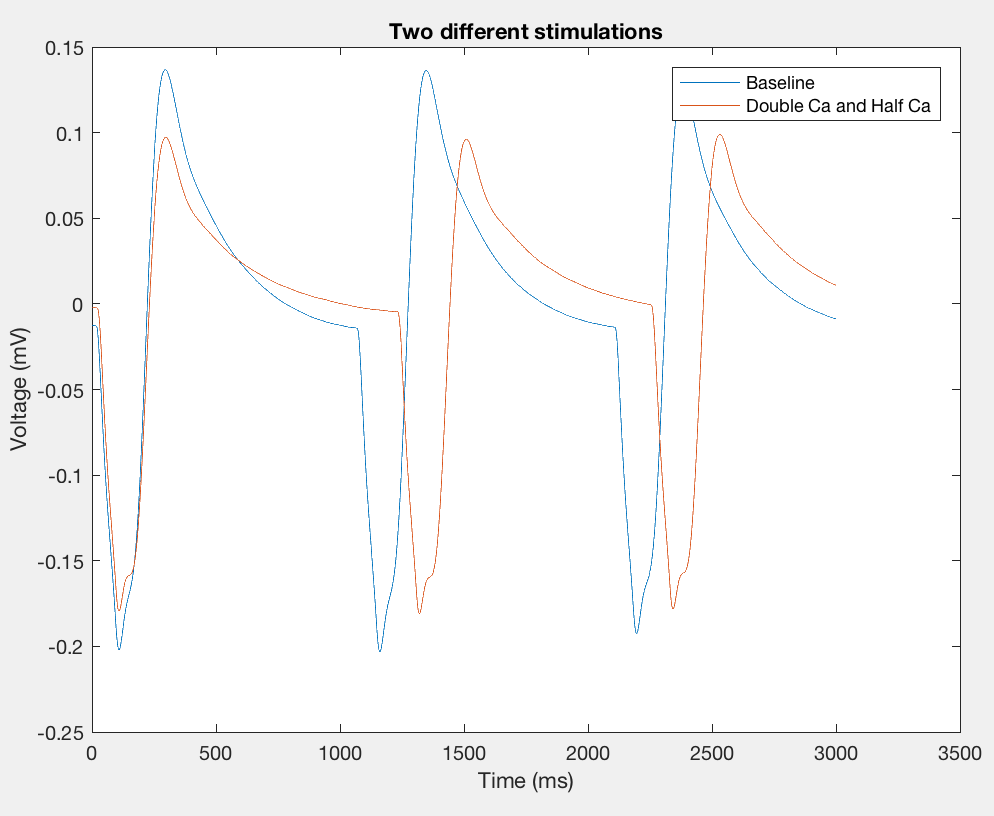
\includegraphics[width = .95\textwidth]{RecInterference.png}
	
	\caption{This figure shows the recording results with the different signals played into the wires at position 2. In one wire the double Ca signal was sent and the other was the half Ca signal. Baseline in Blue, double signal in Red. X axis is time in ms and y is voltage in mV }
	\label{fig:recInterfere}
\end{figure}

%%%%%%%%%%%%%%%%%% Correct Bibliography Style

\bibliography{C:/Users/Jake/Documents/library}
\bibliographystyle{IEEEtran}
*Note a non English citation, but an English translation of the text was obtained and used

\end{document}








